\documentclass[conference]{acmsiggraph}

\TOGonlineid{45678}
\TOGvolume{0}
\TOGnumber{0}
\TOGarticleDOI{1111111.2222222}
\TOGprojectURL{}
\TOGvideoURL{}
\TOGdataURL{}
\TOGcodeURL{}

\title{Ray Tracing Implicit Surfaces}

\author{David Rusk\thanks{e-mail:drusk@uvic.ca}\\University of Victoria}
\pdfauthor{David Rusk}

\keywords{ray tracing, implicit surfaces}

\begin{document}

\maketitle

\begin{abstract}

Write abstract here. \cite{KalraBarr1989}

\end{abstract}

\keywordlist

%% Use this only if you're preparing a technical paper to be published in the 
%% ACM 'Transactions on Graphics' journal.

\TOGlinkslist

%% Required for all content. 

\copyrightspace

\section{Introduction}

Write introduction here.

\section{Background}

Write background here.

\section{Methodology}

Write methodology here.

\section{User Interface}

Write interface description here.

\section{Data Structures}

Write data structures description here.

\section{Algorithms}

Write algorithms description here.

\section{Implementation}

Write about implementation here.

\section{Results}

Write about results here.

\section{Conclusion}

Write conclusion here.

\section{Future Work}

A major area of future work is calculating the Lipschitz constants L and G
for other useful implicit functions.  Kalra and Barr \cite{KalraBarr1989} 
mention a forthcoming report with additional Lipschitz constants, but to
our knowledge no report was ever published.  This will allow new types of
surfaces to be rendered, and greatly increase the utility of implicit 
surfaces for modelling when using ray tracing.

Future development of the application could add support for blending surfaces
which are close to each other.  A simple two-dimensional example of this concept
is shown below.

\begin{figure}[ht]
  \centering
  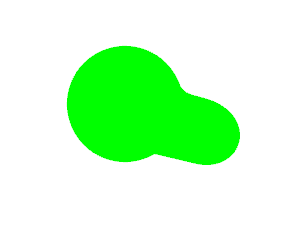
\includegraphics[width=1.5in]{figures/blend2d.png}
  \caption{Two-dimensional blend of two circles.}
\end{figure}

Adding constructive solid geometry (CSG) operations would also be useful
for modelling more advanced structures.  CSG combines primitives like 
spheres and cylinders by using the boolean set operations union,
intersection and difference.

\bibliographystyle{acmsiggraph}
\bibliography{ImplicitSurfacesRayTracer}
\end{document}

